\section{Diagnosing Foundation-Model Relationships for Fusion}
To understand why different foundation-model compositions lead to different fusion performance, we analyze encoder relationships at three complementary levels: global representation geometry, feature-wise statistical association, and task-conditioned encoder attribution and pairwise interaction.
\subsection{Representation Geometry Reveals Non-uniform Similarity Structures}
\begin{figure}[!ht]
    \centering
    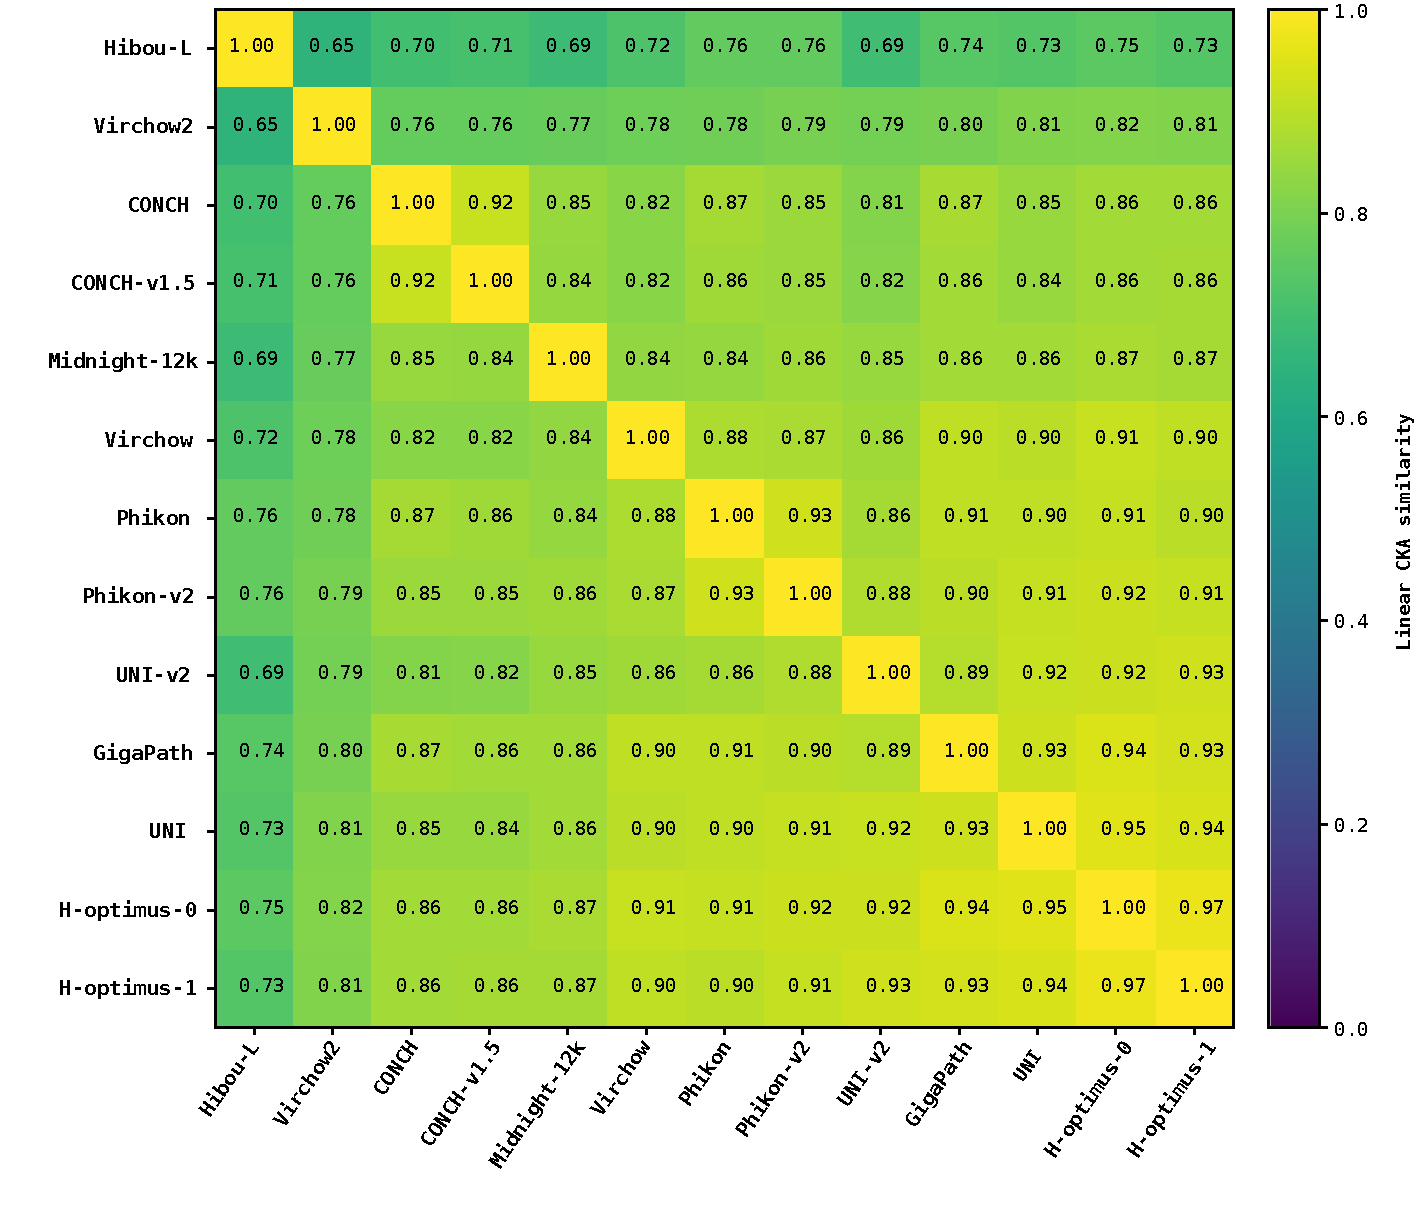
\includegraphics[width=0.8\linewidth]{figs/um_fm/foundation_model_cka_heatmap.pdf}
    \caption{Representation similarity structures among pathology foundation models measured by Linear CKA.}
    \label{fig:cka_heatmap}
\end{figure}

We investigate representation geometry by computing coordinate-aligned linear CKA between encoder pairs (Figure~\ref{fig:cka_heatmap}).
The analysis results reveal non-uniform similarity structures: CKA values range from 0.65 to 0.97, with encoders exhibiting varied representation profiles.
Hierarchical clustering (Appendix Figure~\ref{fig:cka_dendrogram}) further reveals non-uniform grouping structures across the 13 foundation models:
1. Hibou-L and Virchow2 form relatively distinct branches, exhibiting lower CKA similarity with other models.
2. CONCH, Phikon, UNI, GigaPath, and H-optimus share more similar feature spaces, with fine-grained sub-clusters among model variants.

While CKA measures global geometric similarity, it does not reveal feature-level statistical dependencies.
We therefore compute cross-feature Spearman correlations between encoder pairs using coordinate-aligned patches.
Let \(\mathbf{X}_{m}^{(n)}\in\mathbb{R}^{P_n\times d_m}\) denote the embedding matrix produced by encoder \(m\) for slide \(n\), where \(P_n\) is the number of spatially aligned patches and \(d_m\) is the embedding dimension of encoder \(m\).
For the \(a\)-th feature of encoder \(i\) and the \(b\)-th feature of encoder \(j\), we define

\begin{equation}
   \mathbf{x}^{(n)}_{m,a} = \mathbf{X}^{(n)}_{m}[:,a] \in\mathbb{R}^{P_n}.
\end{equation}
The Spearman rank correlation across aligned patches is then computed as
\begin{equation}
    \rho_{ijab}^{(n)}
    =
    \operatorname{corr}
    \left(
    \operatorname{rank}\big(\mathbf{x}^{(n)}_{i,a}\big),
    \operatorname{rank}\big(\mathbf{x}^{(n)}_{j,b}\big)
    \right).
\end{equation}

Each encoder pair \(i, j\) yields \(d_i d_j\) cross-feature correlations for slide \(n\).
We summarize the feature-level statistical association between the two encoders by averaging the absolute correlations over all feature pairs and slides:

\begin{equation}
    R_{ij}
    =
    \frac{1}{N}
    \sum_{n=1}^{N}
    \left[
    \frac{1}{d_i d_j}
    \sum_{a=1}^{d_i}
    \sum_{b=1}^{d_j}
    \left|\rho_{ijab}^{(n)}\right|
    \right]
\end{equation}

The absolute value measures the strength of monotonic association regardless of correlation direction.
Finally, to quantify the relationship between CKA-based representation similarity and feature-wise statistical association, let \(\overline{C}_{ij}\) denote the slide-averaged Linear CKA between encoders \(i\) and \(j\), and let \(R_{ij}\) denote their mean absolute feature-wise Spearman association.
We collect all unique encoder pairs from the upper-triangular part of the pairwise matrices (\(i<j\)) and compute:

\begin{equation}
    \rho_{\mathrm{CKA\text{-}FS}}
    =
    \operatorname{Spearman}
    \left(
    \left\{\overline{C}_{ij}\right\}_{i<j},
    \left\{R_{ij}\right\}_{i<j}
    \right)
\end{equation}

This statistic measures the rank-order association between global representation similarity and feature-wise statistical association.
We observe a weak negative rank association between global representation similarity and mean absolute cross-feature Spearman association (Appendix Figure~\ref{fig:all_Spearman_heatmap}).
This association suggests that, for the evaluated encoder compositions, geometric representation similarity and cross-feature statistical association capture different aspects of encoder relationships.

\subsection{Variation in Fusion Performance Across Representation Compositions}
Although foundation models exhibit diverse representation structures, it remains unclear whether increasing the number of integrated encoders alone can reliably improve fusion performance.
We observe non-monotonic and method-dependent trends: adding an encoder may improve performance under one representation composition while providing limited benefit or degradation under another.
Therefore, encoder quantity alone is insufficient to explain fusion behavior; effective fusion requires understanding representation composition.
Detailed experimental results are discussed in Section~\ref{scaling law section}.

\subsection{Sample-specific Encoder Contributions Motivate Adaptive Routing}
While representation-level and feature-level relationships characterize encoder similarities, they do not quantify whether an encoder improves downstream task performance when added to a multi-encoder fusion.
Therefore, we perform task-driven analysis to quantify the variation in encoder-specific contributions across individual slides.
We adopt a leave-one-encoder-out (LOO) attribution strategy, where the representation of the held-out encoder is replaced with an encoder-specific mean baseline.
For a trained reference classifier using the complete encoder set \(\mathcal{E}\), let \(f_y(\mathcal{E}^{(n)})\) denote the target-class one-vs-rest logit margin for slide \(n\). 
For encoder \(m\), its LOO attribution is defined as:
\begin{equation}
    C_m^{\mathrm{LOO}}(n)
    =
    f_y\big(\mathcal{E}^{(n)}\big)
    -
    f_y\big(\mathcal{E}_{\setminus m}^{(n)}\big),
\end{equation}
where \(\mathcal{E}_{\setminus m}^{(n)}\) denotes the encoder set in which the embedding of encoder \(m\) is replaced by an encoder-specific mean baseline, while the representations of all other encoders remain unchanged.
The LOO analysis reveals that different foundation models exhibit distinct contribution patterns across samples.
To further investigate whether encoder pairs exhibit non-additive interactions, we extend the analysis to pairwise task-level interaction.
For a pair of encoders $(i,j)$, we define the pairwise interaction attribution as:
\begin{equation}
    I_{ij}(n)
    =
    f_y(\mathcal{E}^{(n)})
    -
    f_y(\mathcal{E}_{\setminus i}^{(n)})
    -
    f_y(\mathcal{E}_{\setminus j}^{(n)})
    +
    f_y(\mathcal{E}_{\setminus \{i,j\}}^{(n)})
\end{equation}
This inclusion--exclusion score quantifies the non-additive task-specific interaction between two encoders, where positive and negative values indicate synergistic and interfering effects, respectively.
The LOO attribution and pairwise interaction analyses provide offline diagnostic evidence motivating adaptive routing.
The interaction analysis further suggests that representation similarity does not always align with task-level interaction (Appendix Figure~\ref{fig:n5_high_redundancy_quadrants}).
Therefore, representation similarity alone may not fully characterize encoder redundancy, motivating adaptive routing that accounts for encoder utility at the sample level.